\documentclass{beamer}

\usepackage{amsmath, amssymb}
\usepackage{tikz-cd}
\usepackage{xcolor}
\usepackage{graphicx}

\title{MAT434: Theory of Mathematical Statistics}
\author{\textbf{Miraj Samarakkody}}
\institute{Tougaloo College}
\date{03/31/2025}

\begin{document}

\begin{frame}
    \titlepage
\end{frame}








\begin{frame}{Chapter 3}
 \Huge{Discrete Random Variables}
\end{frame}



\begin{frame}{Discrete Random Variables}
    Suppose that \(X\) and \(Y\) are discrete random variables defined on the same sample space and that they take on values \(x_1,x_2, \dots\), and \(y_1,y_2, \dots\) respectively. \\ \pause
    \vspace{0.1in}

    Their \textbf{joint frequency function} \(p(x,y)\) is \[
    p(x_i, y_j) =P(X=x_i, Y=y_j)
    \]
\end{frame}

\begin{frame}{Example}
    A fair coin is tossed three times and let \(X\) denote the number of heads on the first toss and \(Y\) the total number of heads. Find joint frequency function of \(X\) and \(Y\).  \\ \pause
    \vspace{0.2in}
    Find the frequency function of \(Y\) \((p_Y)\) from the joint frequency function. \\ \pause
    \vspace{0.2in}
    The \(p_Y\) is called the \textbf{marginal frequency function} of \(Y\). 
\end{frame}

\begin{frame}{Marginal Frequency Function}
Let \(X\) and \(Y\) are discrete random variables defined on the same sample space. The marginal function of \(X\) can be written as 
\[p_X(x)= \sum_i p(x,y_i)\] In the similary way, we can write the marginal frequency function for \(Y\).
\end{frame}

\begin{frame}{Multinomial Distribution}

    \begin{itemize}
        \item This is a generalization of the binomial distribution. \\ \pause
    \item Suppose that each of \(n\) independent trials can result in one of \(r\) types of outcomes and that one each trial the probabilities of the \(r\) outcomes are \(p_1,p_2, \dots, p_r\). \\ \pause
     \item Let \(N_i\) be the total number of outcomes of type \(i\) in the \(n\) trials, \(i=1, \dots, r\). \\ \pause

    \item We observe that any particular sequence of trials giving rise to \(N_1=n_1, N_2=n_2, \dots, N_r=n_r\) occurs with probability \(p_1^{n_1} p_2^{n_2}\dots p_r^{n_r}\)\\ \pause

    \item There are \(\dfrac{n!}{n_1!n_2!\dots n_r!}\) such sequences. \\ \pause

    \item Thus the joint frequency function is \[p(n_1,n_2,\dots,n_r)= \begin{pmatrix}
        n \\
        n_1n_2\dots n_r
    \end{pmatrix} p_1^{n_1}p_2^{n_2}\dots p_r^{n_r}\]
\end{itemize}
\end{frame}

\begin{frame}{Multinomial Distribution}

\begin{itemize}

    \item The marginal distribution of any particular \(N_i\) can be obtained by summing the joint frequency function over the other \(n_j\). \\ \pause
    \item This tedious calculations can be avoided. \\ \pause
    \item Note that \(N_i\) can be interpreted as the number of successes in \(n\) trials, each of which has probability \(p_i\) of success and \(1-p_i\) of failure. 
    \item Therefore, \(N_i\) is a binomial random variable, and \[p_{N_i}(n_i)=\begin{pmatrix}
        n\\
        n_i
    \end{pmatrix} p_i^{n_i}(1-p_i)^{n-n_i}\]
    
\end{itemize}
\end{frame}

\begin{frame}{Chapter 3}
    \Huge{Continuous Random Variables}
\end{frame}

\begin{frame}{Continuous Random Variables}
    \begin{itemize}
        \item Suppose that \(X\) and \(Y\) are continuous random variables with a joint cdf, \(F(x,y)\). \pause
        \item Their \textbf{joint density function} is a piecewise continuous function of two variables, \(f(x,y)\). \pause
        \item The density function \(f(x,y)\) is non-negative and \(\int_{-\infty}^{\infty} \int_{-\infty}^{\infty} f(x,y)~dy~dx=1\). \pause
        \item For two dimensional set \(A\) \[P((X,Y) \in A)= \iint_A f(x,y)~dy~dx\]
    \end{itemize}
\end{frame}

\begin{frame}{Continuous Random Variable}
    \begin{itemize}
        \item In particular, if \(A=\{(X,Y)|X \leq x \text{ and }Y \leq y\}\), \[F(x,y) \int_{-\infty}^x \int_{-\infty}^{y} f(u,v)~dv~du\]\pause
        \item From the fundamental theorem of multivariable calculus, \[f(x,y)= \dfrac{\partial^2}{\partial x \partial y}F(x,y)\]
    \end{itemize}
\end{frame}

\begin{frame}{Example A}
    Consider the bivariate density function \[f(x,y)=\dfrac{12}{7}(x^2+xy),~0 \leq x \leq 1,~0\leq y \leq 1.\] Calculate \(P(X>Y)\). 

    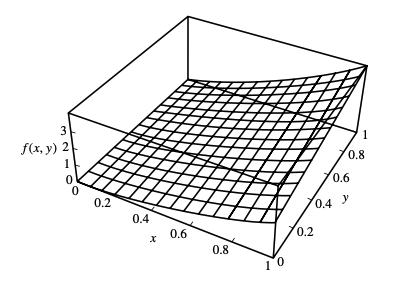
\includegraphics[scale=0.5]{Figures/fig_7.png}


\end{frame}

\begin{frame}{Continuous Random Variables}
    The \textbf{marginal cdf} of \(X\), of \(F_X\), is \begin{align*}
        F_X(x) & = P(X \leq x)\\
        & = \lim_{y \to \infty}F(x,y)\\
        & = \int_{-\infty}^{x} \int_{-\infty}^{\infty} f(u,y)~dy~du
    \end{align*}
    The marginal density of \(X\) is \[f_X(x)=F'_X(x)= \int_{-\infty}^{\infty}f(x,y)~dy\]
\end{frame}


\begin{frame}{Example B}
    Consider the bivariate density function \[f(x,y)=\dfrac{12}{7}(x^2+xy),~0 \leq x \leq 1,~0\leq y \leq 1.\] Find the marginal density of \(X\). 


\end{frame}

\begin{frame}
    \frametitle{Example D}

    Consider the following joint density:
    \[f(x,y)= \begin{cases}
        \lambda^2 e^{-\lambda y}, & 0 \leq x \leq y, ~\lambda >0\\
        0, & \text{elsewhere}
    \end{cases}\] Find the marginal densities. 
    
    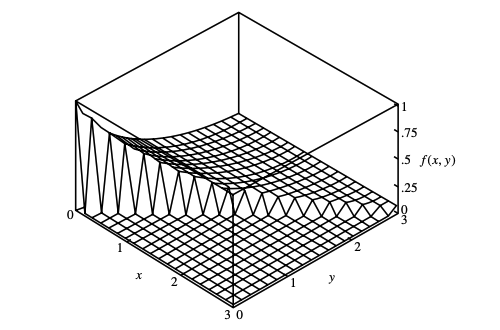
\includegraphics[scale=0.5]{Figures/fig_8.png}

\end{frame}

\begin{frame}{Continuous Random Variables}
    \begin{itemize}
        \item In some applications, it is useful to analyze distributions that are uniform over some region space. 
        \item For example, in the plane, the random point \((X,Y)\) is uniform over a region \(R\), if for any \(A \subset R\), \[P((X,Y) \in A)=\dfrac{|A|}{|R|}\]
    \end{itemize}    
\end{frame}

\begin{frame}{Example E}
    A point is chosen randomly in a disk of radius 1. Since the area of the disk is \(\pi\), \[f(x,y)= \begin{cases}
        \dfrac{1}{\pi} & \text{if }x^2+y^2\leq 1\\
        0, & \text{otherwise}
    \end{cases}\] Find \(F_R(r)\), \(f_R(r)\)  \(f_X(x)\) and \(f_Y(y)\). 
\end{frame}
\end{document}